\chapter{Client Side}
\paragraph{}
This chapter discusses the client side of WebSlicer in detail. 
It also includes some necessary background about AngularJS as it will be crucial to understanding latter sections of this chapter.

\section{AngularJS}
\paragraph{}
In order to understand the structure of WebSlicer a few things must be known about how AngularJS applications are structured and how AngularJS itself works.
\subsection{Controllers \& Data Binding}
\paragraph{}
The controller structure in AngularJS that sits between the view and the JavaScript world acts like the glue between the two.
From a controller the user is allowed access to ``scope'' variables, which are similar to normal JavaScript variables, but they have a special two-way data binding property.
Two-way data binding is one of the most interesting features of AngularJS, as it gives the user real time updates as the user interacts with a view.
In traditional JavaScript, a developer must identify key events that occur in the browser as the trigger for a sequence of events.
AngularJS also has a sequence of events but no trigger is required as the sequence of events is triggered automatically.
This action is known as a digest cycle.
AngularJS has a watch function for each variable attached to its scope.
When any changes to this variable occur, they propagate that change to the functions that are associated with that variable \citep{freeman-2014}.

\subsection{Factories \& Services}
\paragraph{}
JavaScript has many pitfalls, including the lack of any kind of larger design pattern support, such as Object Oriented Programming (OOP).
The current trend with web based applications is to create single page applications with the same functionality as prior designs that have many pages.
AngularJS is the answer to this with Factories and Services which mimic the design of a POJO (Plain Old Java Object) and Singleton objects in Java.

\subsection{Directives}
\paragraph{}
A directive is one of the most powerful structures in AngularJS.
It allows the programmer the power to write their own HTML5 tag with its own parameters and rules.
Directives also contain support for templates which are HTML snippets that replace the main tag when the code is loaded.
Combining this with the use of the aforementioned design patterns creates a very powerful tool to create and organize dynamic content.

\section{WebSlicer AngularJS Structure}
\paragraph{}
This section discusses the entire client side structure of WebSlicer when it is broken down into its respective Controllers, Factories, and Directives.

% this figure describes my full angular structure on the client
\begin{figure}[!ht]
  \centering
  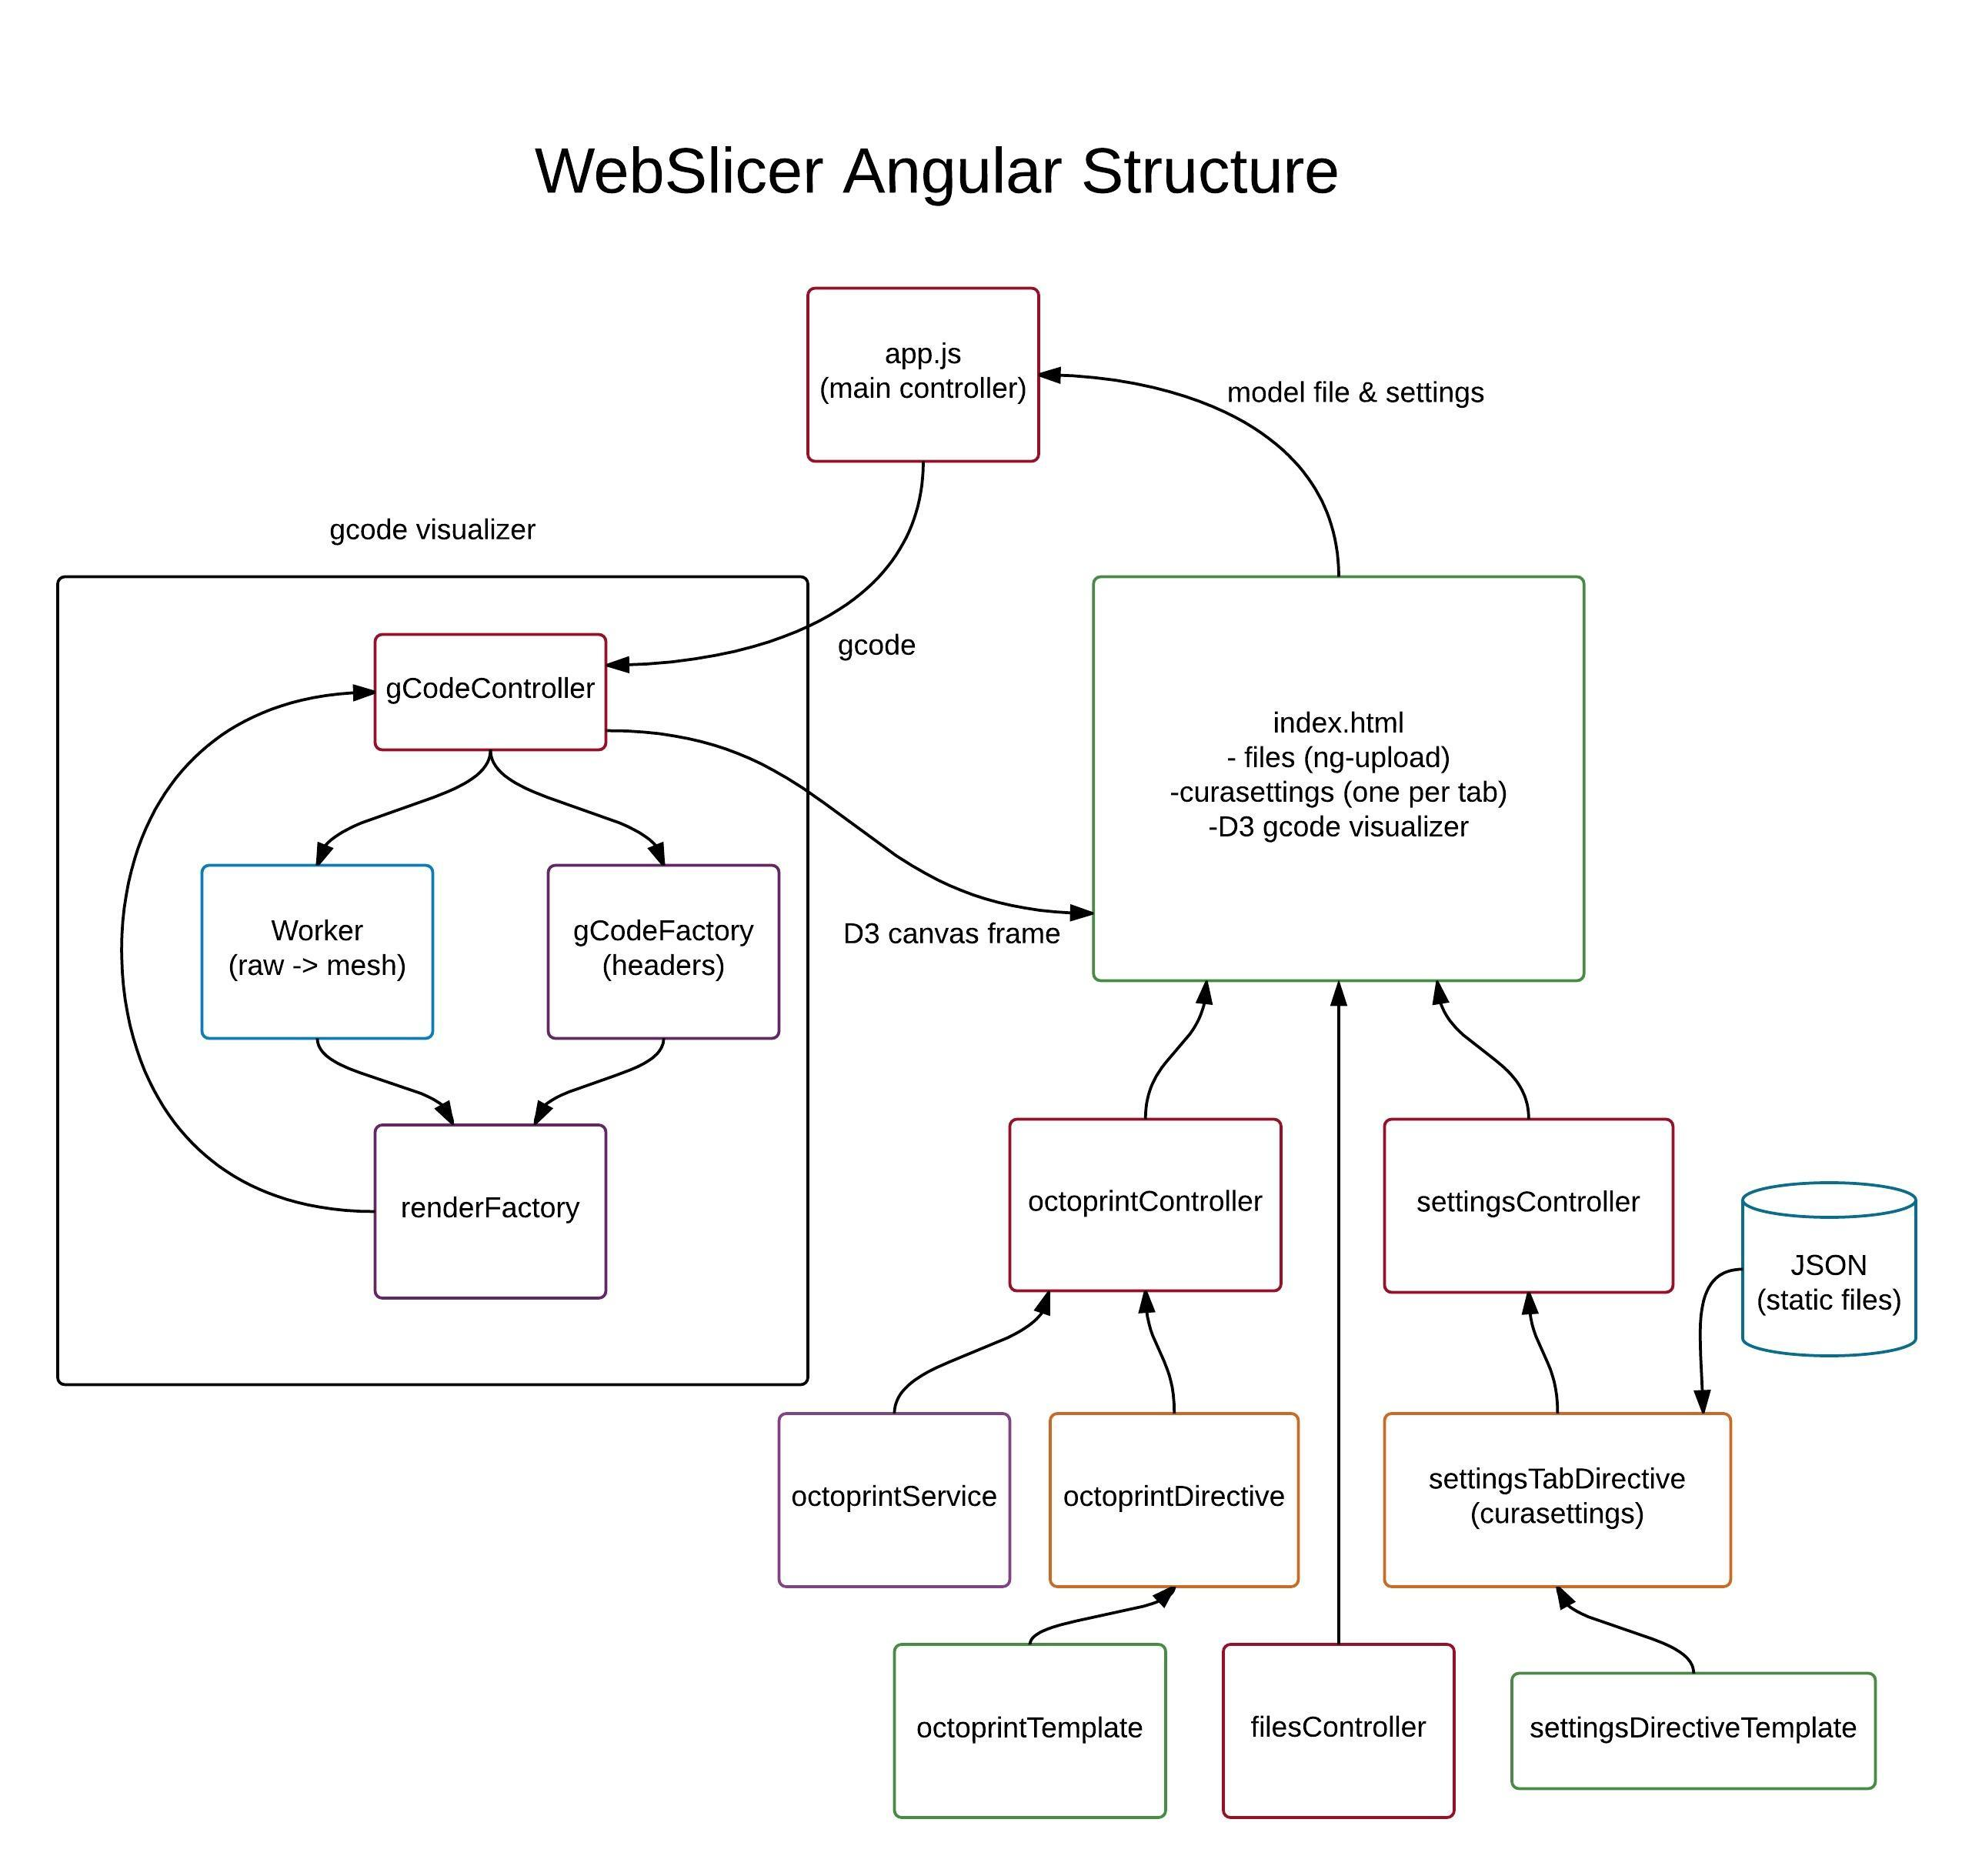
\includegraphics[width=\linewidth]{diagrams/Client-Side-Structure}
  \caption{Full AngularJS structure breakdown}
  \label{fig:client-side-structure}
\end{figure}

\subsection{app.js}%app.js
\paragraph{}
The full graphical AngularJS structure of WebSlicer is shown in Figure \ref{fig:client-side-structure}.
Flow through this diagram starts with the app.js node which represents the main controller of the application.
This can be thought of as a main function in C++.
The main control variables are also inside of app.js which are similar to global variables.
Variables in this controller are used to store the current settings, file pointer, and output G-code.

\subsection{index.html}%index.html
\paragraph{}
Figure \ref{fig:client-side-structure} also shows that index.html is large hub and, as WebSlicer is a single page web application, this is the only static HTML file.
Index.html has several other functions, such as bringing in all libraries and custom directives.

\subsection{Settings}%settings
% the flow of a settings throguh the application
\begin{figure}[!ht]
  \centering
  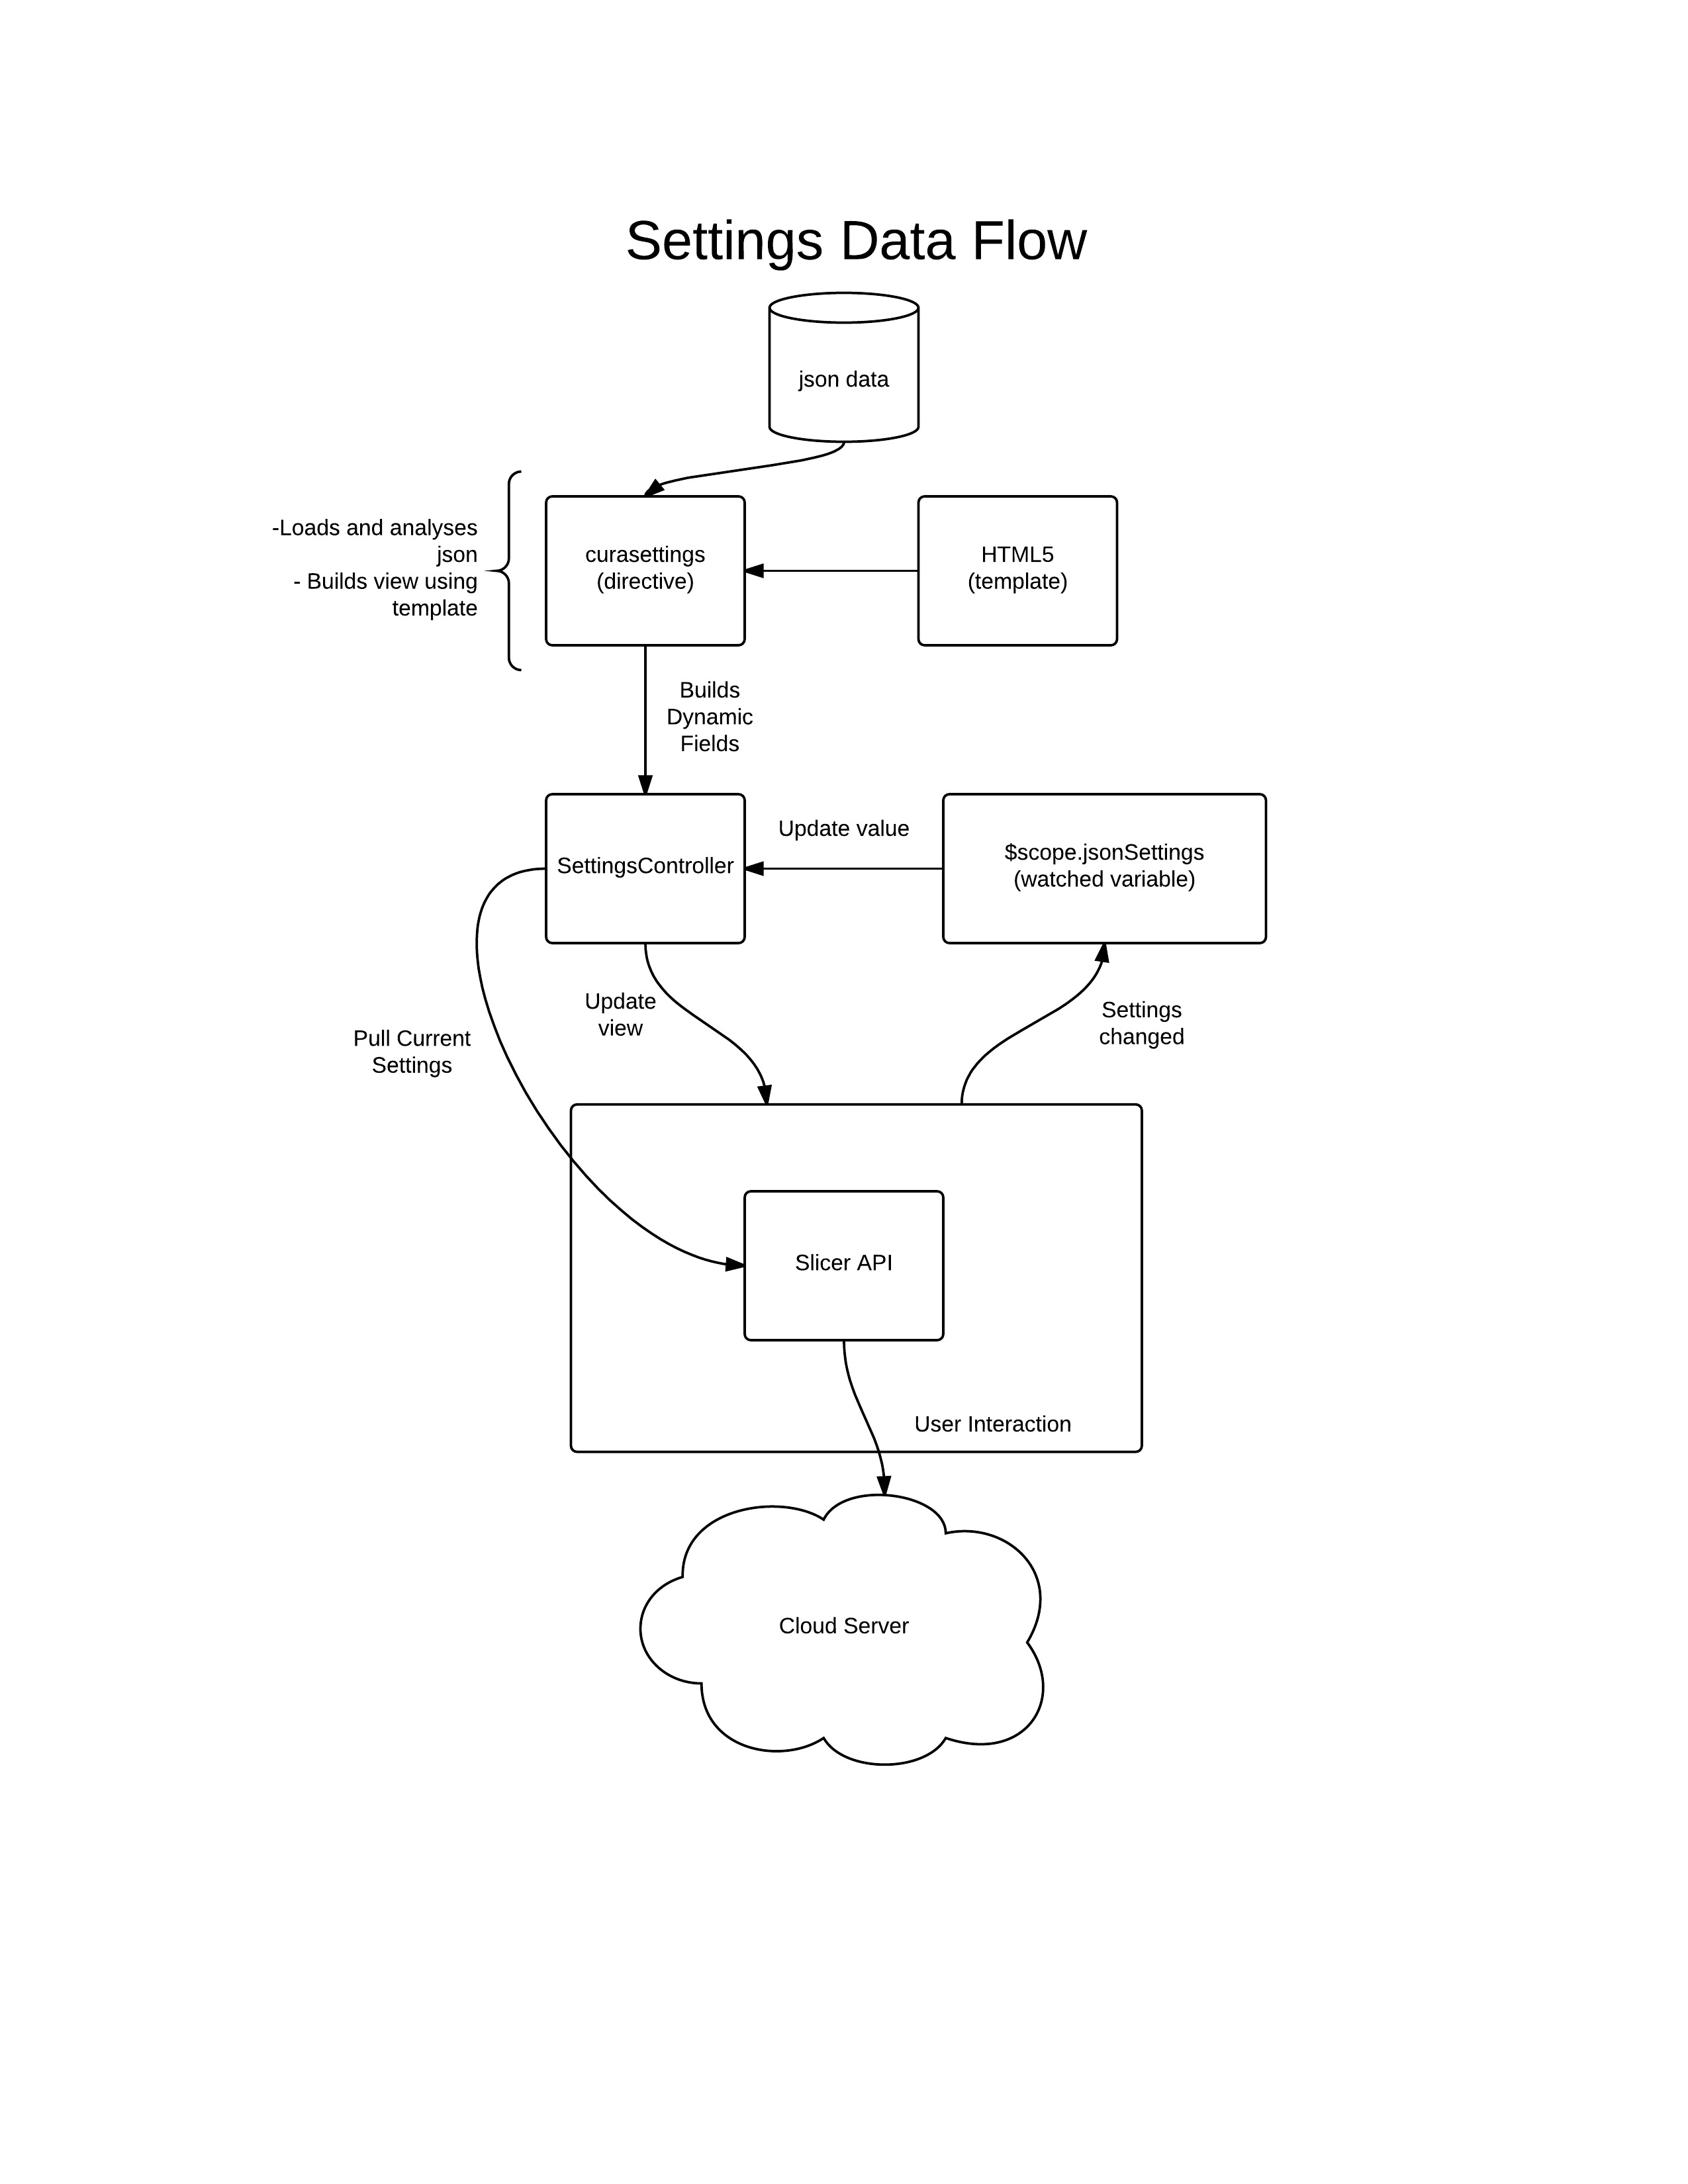
\includegraphics[width=\linewidth]{diagrams/Settings-Data-Flow}
  \caption{The flow of data through the application from beginning to end of client side user interaction}
  \label{fig:settings-data-flow}
\end{figure}
\paragraph{}
As shown in Figure \ref{fig:settings-data-flow}, settings have a long path that they must travel before they are submitted to be used while slicing. 
This data flow starts with loading a static JavaScript Object Notation (JSON) file, which describes the settings in a pattern as shown in Listing \ref{lst:json-settings}.

% JSON settings example listing
\lstsetjavascript
\begin{lstlisting}[language=json, label={lst:json-settings}, caption=A sample from a static settings file in JSON format.]
{
    "setting": "layer_height",
    "default": 0.1,
    "type": "float",
    "category": "Quality",
    "label": "Layer Height (mm)",
    "description": "Layer height in millimeters. This is the most important setting to determine the quality of your print. Normal quality prints are 0.1mm, high quality is 0.06mm. You can go up to 0.25mm."
}
\end{lstlisting}

% HTML example for how ng-repeat works
\lstsetxml
\begin{lstlisting}[language=HTML5, label={lst:html-repeat-example}, caption=An example of a ng-repeat looping construct in HTML5.]
<table class="table">
	<tr><td>Action</td><td>Done</td></tr>
	<tr ng-repeat="item in todos">
		<td>{{item.action}}</td>
		<td>{{item.done}}</td>
	</tr>
</table>
\end{lstlisting}

\paragraph{}
A directive called curasettings takes this static JSON file and divides it so an input field exists in the template for each setting object.
AngularJS provides this functionality through the use of an ng-repeat, which is written in a similar fashion to that of a for-loop in Python which is shown in Listing \ref{lst:html-repeat-example}.
Using a template for a directive in this case also means that the user can have control over many different fields, such as drop-downs and number-specific inputs.
The curasettings directive also gave the logical separation of one static JSON file per tab of settings in the UI, which made it simple to find and modify the settings as needed.

\paragraph{}
Settings in WebSlicer have a complex method of being tracked after loading to the client.
In most applications such as this, there would be an individual watch on each field or a submit button which would trigger grabbing all the fields.
WebSlicer, however, uses a single object to track all of the settings for the application and uses a dynamic method of AngularJS to map from the input field to a field of a single object.
Thus, when the settings are submitted, there is no more interpolation needed, as the settings object already has the current state as shown in the Figure \ref{fig:settings-data-flow} as ``Pull Current Settings.''

\subsection{G-code Visualizer}
\paragraph{}
The G-code visualizer is a layer-by-layer G-code analyzer to aid in model slicing.
It is written using a combination of D3 and a JavaScript web worker.
From Figure \ref{fig:client-side-structure}, it can be seen that the controller for the visualizer is sent in a G-code file, which it splits up to two separate services.
The controller completes an initial parse of the file, which places each one of the lines into its own entry in an array before exchanging it with gCodeFactory and Worker.
Both of these files parse through this entire array, but do so at roughly the same time to expedite the process of visualizing.
The worker takes the array of lines and ignores the header to just focus on converting the raw movement commands into D3 lines so that they may be rendered.
The gCodeFactory takes the headers from the array and uses them to do analytics of the G-code file, such as total print time.

\paragraph{}
The final steps in the process of visualizing the G-code require splitting the G-code file into layers for rendering.
This task which is made simple by following the given tags in the G-code which signal a layer change.
Once all of the cumbersome tasks of parsing and splitting up the G-code file are finished, it is simply a matter of returning layer requests with canvas frames.
Each time a layer is requested, a progress for that layer is also sent.
The controller then indexes to the layer height in the array and renders a frame with the number of lines that are described by the current progress.
As array indexing is nearly instantaneous, the visualizer once parsed and loaded runs very quickly to display layers.

\section{Key Challenges}
\paragraph{}
Discussed in this section were the most notable challenges that had to be overcome when developing the client side of WebSlicer.

\subsection{Visualizer Integration}
\paragraph{}
The visualizer starter code for this was originally written by Nils Hitze as an open source project which had many other features \citep{hitzeViewer-2015}.
This code, however, required a lot of work to integrate properly with the rest of the application.
AngularJS, despite its many features does not mix well with other projects.
Ultimately, the only code that remained from the original was the JavaScript web worker and some of the parser code.

\subsection{Interpolating Settings}
\paragraph{}
A method was required to be designed for the application to handle a lot of input fields.
A simpler method would have been to create a series of fields, each with their own variable, and submit methods and triggers; however, if settings ever change format it would require refactoring many files.
Thus, spending the extra time to design an intelligent method of handing large amounts of input data seemed logical.
This, however, took much more time and effort than anticipated.
%explain this event more
At one point, this even required contacting the original developers of CuraEngine discuss the meaning of some of their settings.
Documentation for many of the settings was dissatisfactory and in many instances was non existent which further slowed down development.

\section{Other Planned Integrations}
\paragraph{}
During the development process often many items do not make it into the final product for various reasons.
Included in this section are some items which were cut from WebSlicer before beta testing.

\subsection{OctoPrint}
\paragraph{}
A feature that was removed at a late state in the process of building this application was an integration with OctoPrint.
OctoPrint has a exceptional API that allows for external applications to integrate easily, making it an ideal choice for this application.
This integration was to allow a user who was running an OctoPrint server to be able to send files directly to their server.
This would eliminate the need to download the G-code from WebSlicer only to be uploaded to the print server seconds later.
It was decided at the last moment that this feature need not be in the minimum viable product and that time was best allocated to finishing more crucial features of the application.

\subsection{Thingiverse \& YouMagine}
\paragraph{}
Another planned integration was the ability to import from a web based repository such as Thingiverse or YouMagine.
These repositories are public sites where users can upload their 3D designs so others can 3D print them.
Thingiverse in particular has a effective API for accessing models from their site, which would make it an easy integration for a web based slicing software;
however, this feature was terminated early on, as it would have required too much unnecessary development time to finish.

\section{Issues \& Known Bugs}
\paragraph{}
As mentioned in prior sections, WebSlicer was designed with a minimum viable product in mind.
Developing a working 3D print slicer for the web was the primary task and all other features needed to support this or extend this functionality.
For this reason, there is no login or user database, which would normally be the first item to be developed for an application such as this.
There is also no way to view any of the models in 3D which, as discussed in latter sections of this thesis, makes the software harder to use.
